\subsection{Production}

Im Gegensatz zu einem Research Honeypot wird ein Production Honeypot, wie der Name schon sagt, in einem produktiven Umfeld eingesetzt. 
\\
\begin{figure}[ht]
    \centering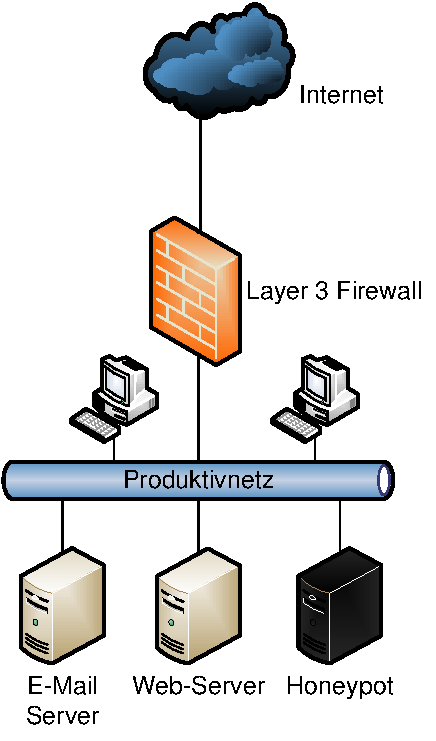
\includegraphics[scale=0.6]{Bilder/produktiv.pdf}
  \caption{Research Honeypot}
  \label{hnet:geni}
\end{figure}
\\
\begin{itemize}							% Beginn der Aufzählungsumgebung
\item{\textbf{Prevention}} \\ asdasda sfs				
\item{\textbf{Detection}} \\
\item{\textbf{Response}} \\
\end{itemize}